\section{How did you experience Neil Armstrong's first steps on the moon?}
My response to this question is a reflection that includes memories of how our family learned the news from our community and around the world.
We received a daily newspaper and the most interesting pages for me were the wedding and engagement announcements second only to the comic's page.
I had a vague feeling that reading the comic page was not approved of by the parents but I have no memory of being told not to read the cartoons.

Another source of news was the Life magazine that my Aunt Anna subscribed to.
We visited the three Aunties most often on Friday evenings.
The evening visit often included watching Aunt Dorothy's latest slide show that was full of familiar scenes and people from around our community.
I believe she enjoyed her role as the photographer of the family.
Then there was the pictures in the magazine rack next to Aunt Anna's chair full of past and recent Life magazines to look at.
My memories of learning about men landing on the moon involved seeing the pictures published there.
\begin{figure}
\centering
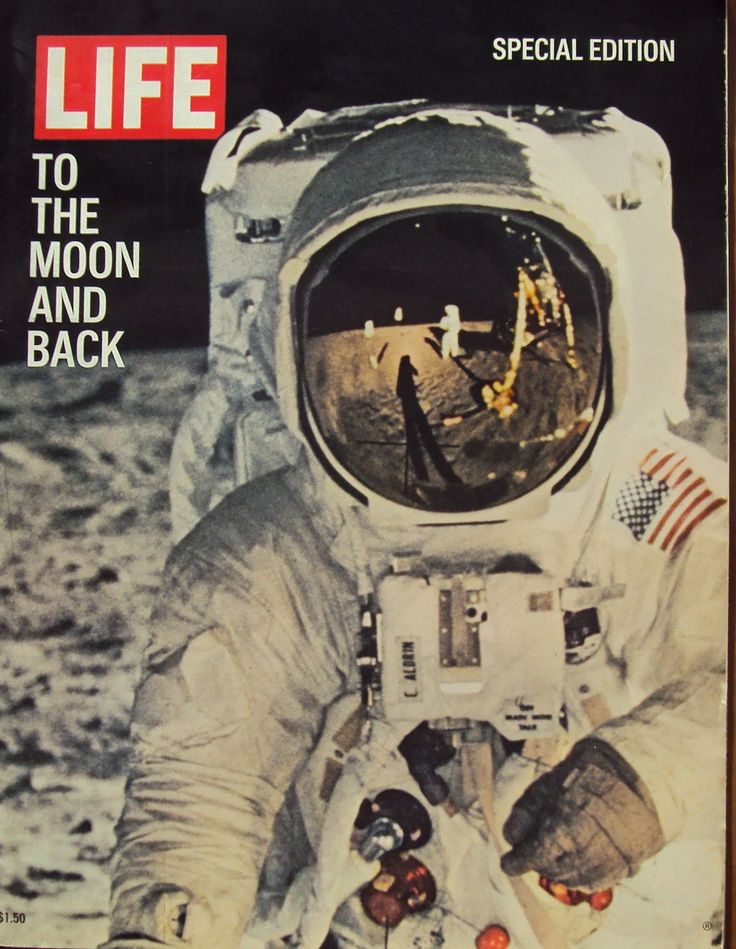
\includegraphics[width=0.9\textwidth]{finding_my_way/2.jpg}
\caption{
Landing on the moon
}
\end{figure}

Life magazine opened up a world far from the farming community in which I grew up.
I remember looking at the moon in the night sky, amazed and wondering if that really was the place that the moon landing pictures were taken.

From Tim - I love this image of you looking up at the moon in the night sky.
Also, are Aunt Dorothy's photographs collected anywhere?
From Mom - No unfortunately they are not in one location and I believe that many were destroyed.
I have a collection of them that I picked out the day of the Aunties house was emptied and sold at auction.
I was not invited to be involved with decisions about Aunt Dorothy's slides.
I might have suggested something different than scattering them among the nieces and nephews and discarding what remained.
Than again it was not easy to know what to do with them.






